\documentclass[11pt]{article}
\usepackage{isma2018}

% Enter further packages required for your manuscript below.
\usepackage{graphicx}
\usepackage{caption}
\usepackage{subcaption}
%%%%%%%%%%%%%%%%%%%%%%%%%%%%%%%%%%%%%%%%%%%%%%%%%%%%%%%%%%%%%%%%%%%
% The "hyperref" package may be used in conjunction with PDFLatex %
% to add document information to the generated PDF file. Please,  %
% fill out the same title, author(s) and keywords as on the paper %
% submission form. Note, that the "hypperref" package should be   %
% loaded as the last.                                             %
%                                                                 %
% If you are not using PDFLatex, delete or comment the following  %
% lines. In that case, the conference secretary will add the      %
% document information to your PDF file.                          %
%%%%%%%%%%%%%%%%%%%%%%%%%%%%%%%%%%%%%%%%%%%%%%%%%%%%%%%%%%%%%%%%%%%

\usepackage[pdftex]{hyperref}
\hypersetup{a4paper = true,
	pdfpagemode = None,
	pdfstartview  = FitH,
	citebordercolor = 1 1 1,
	filebordercolor = 1 1 1,
	linkbordercolor = 1 1 1,
	urlbordercolor = 1 1 1}
\hypersetup{pdftitle  = {Manuscript preparation instructions},
	pdfauthor = {A. Michalak,  A. Wy{\l}oma{\'n}ska, J. Wodecki,  R. Zimroz, K. Gryllias},
	pdfkeywords = {local damage detection, vibration signal analysis, ADF test}}


\usepackage[numbers,square,sort&compress]{natbib}
\usepackage{color}


\title{Optimal frequency band selection via stationarity testing in time frequency domain}

\author{\textbf{A. Michalak $^1$,  A. Wy{\l}oma{\'n}ska $^1$, J. Wodecki $^1$,  R. Zimroz $^2$, K. Gryllias $^{3,~4}$} \\
  $^1$  KGHM Cuprum Ltd, Research and Development Centre,\\ 
  Sikorskiego 2-8, 53-659 Wroc{\l}aw, Poland  \\
%   e-mail: \textbf{\{amichalak, awylomanska, jwodecki\}@cuprum.wroc.pl} 
% % Uncomment this block to add multiple (different) affiliations.
 \\
  $^2$ Faculty of Geoengineering, Mining and Geology, Diagnostics and Vibro-Acoustic Science Laboratory, Wroc{\l}aw University of Science and Technology,\\
  Na Grobli 15, 50-421 Wroc{\l}aw, Poland \\
%   e-mail: \textbf{radoslaw.zimroz@pwr.wroc.pl} 
  \\
  $^3$ KU Leuven, Department of Mechanical Engineering, \\
  Celestijnenlaan 300 - box 2420, 3001 Leuven, Belgium \\
  \\ 
  $^4$ Dynamics of Mechanical and Mechatronic Systems, Flanders Make, Belgium\\
  \\
  e-mail of Corresponding Author: \textbf{jwodecki@cuprum.wroc.pl} 
  }

\date{}

\begin{document}

\abstract{In the last decades a plethora of signal processing tools have been proposed for the analysis of vibration signals, focusing on fault detection and diagnosis of rotating machinery. Despite the existence of numerous methodologies, there is still a need to construct more specific diagnostic algorithms. The informative frequency band is a purely frequency-domain idea, so very often the approach of spectral selectors is pursued and those are digital filters prepared in a custom way. In this paper a novel signal processing approach is proposed based on the analysis of the time-frequency domain. The vibration signal is firstly transformed to the time-frequency domain. Moreover the stationarity of the time series vectors within the discrete frequency bins of the Time-Frequency (T-F) map is statistically tested by using the Augmented Dickey-Fuller (ADF) test. A frequency band filter selector is then constructed by the aggregation of the ADF statistic values of narrow frequency bins into a vector spanning over the whole Nyquist band of the given signal. }

% \abstract{In the era of Industry 4.0 and smart machines, condition monitoring of rotating machinery plays an important role. In the last decades a plethora of signal processing tools have been proposed for the analysis of vibration signals, focusing towards the early and accurate fault detection and diagnosis of rotating machinery. Some of the existing algorithms are based on the filtering around an informative frequency band, which contains the diagnostic information usually in the form of a modulation of a carrier frequency by a characteristic fault frequency. A number of approaches and experience rules have been proposed during the last decade for the optimum manual or automatic identification and selection of the informative frequency band where usually the Signal-to-Noise Ratio (SNR) is high and the fault is more easily detected. Despite the existence of numerous methodologies, there is still a clear industrial need to construct more specific diagnostic algorithms, since real-life industrial signals are usually non-typical, noisy, complex and difficult to be handled. The informative frequency band is a purely frequency-domain idea, so very often the approach of spectral selectors is pursued and those are, simply speaking, digital filters prepared in a custom way. In this paper a novel signal processing approach is proposed based on the analysis of the time-frequency domain. Following briefly the procedure, the vibration signal is firstly transformed to the time-frequency domain. Moreover the stationarity of the time series vectors within the discrete frequency bins of the Time-Frequency (T-F) map is statistically tested by using the Augmented Dickey-Fuller (ADF) test in order to check if the given signal corresponds to a healthy or a damaged machine. A frequency band filter selector is then constructed by the aggregation of the ADF statistic values of narrow frequency bins into a vector spanning over the whole Nyquist band of the given signal. The filter can be further applied on the vibration signals following classical methodologies, leading to fault detection and diagnosis.}

\maketitle

\section{Introduction}
The notion of introducing so-called \emph{intelligent solutions} for maintenance of industrial machinery drives the need for development of specialized analytical methods for more and more demanding diagnostic scenarios. Machines with rotating components are in the center of research interest due to the high industrial relevance and the high diversity of possible fault cases regarding components interacting with each other. Mechanisms of signal generation by kinematic pairs (e.g. pair of gears) when one of the components is faulty have been studied by many researchers \cite{randall1982new,chaari2008effect,antoni2002differential,antoni2003stochastic}. The fault signature of rolling element bearings may be described as impulsive \cite{antoni2006spectral}, cyclic (or periodic) \cite{michalak2017application}, nonlinear, non-Gaussian \cite{wylomanska2016application}, amplitude/phase modulated \cite{chaari2012gearbox}, etc. Most of these descriptors have been already used as detection criteria - kurtosis was used as a measure of impulsiveness \cite{wodecki2018optimal}, cyclostationary analysis was developed to detect and identify cycles related to damage \cite{wodecki2017informative, kruczek2017multiple} etc. However in this paper the authors propose to use testing of the signal stationarity for machine diagnostics. It is well known, that in case of healthy bearings, a vibration signal measured on the housing will be stationary and will closely follow a Gaussian distribution. In case of local damage, two surfaces in contact will produce a disturbance. Effectively, a series of such impacts in the time domain will manifest itself as a cyclic (or periodic) additive impulsive component. It will definitely introduce disturbance in the signal, which will contribute to the degree of non-stationarity. This observation, made already also by other researchers \cite{martin2007advanced} is the basis for this paper. The key idea here is to test whether the signal is stationary or not and more specifically, instead of evaluating the signal itself, a more structure-oriented approach is proposed. Due to the complexity of machinery and the number of potential sources of non-stationarity, including accidental disturbances \cite{wodecki2017local,zak2017measures}, the test of stationarity will be done in the time-frequency domain, for each frequency bin -- similarly to the Spectral Kurtosis (SK) or to other methods developed for informative frequency band identification. A variety of techniques have been proposed for testing of stationarity of a signal \cite{dickey1979distribution,durbin1951testing,kwiatkowski1992testing}. In this paper the use of the Augmented Dickey-Fuller (ADF) test \cite{dickey1979distribution} is proposed. The distribution of the ADF statistical value along the frequency scale can be estimated and used as a spectral selector similar to SK, being the basis for digital filter characteristic for signal enhancement \cite{obuchowski2014selection}. The approach is validated on real signals captured on pulley bearings. As a further validation step, the results are compared with the SK method in terms of the selector shape as well as of the quality of the obtained filtered signal. The rest of the paper is organised as follows. The methodology is first proposed in Section 2 and it is further applied on real signals and teh results are presented in Section 3. The paper closes with some conclusions in Section 4. 

\section{Methodology}

In this section, the key aspects of the methodology are described. The main idea is to develop a frequency-domain selector based on the spectral stationarity of the signal. The proposed approach in some sense is an extension of the classical methodology based on the Spectral Kurtosis, which is a popular measure of impulsiveness. However the ADF statistic (calculated for each frequency band) is considered here which may indicate the nonstationarity of a subsignal corresponding to a given frequency band. The flowchart of the proposed algorithm is presented in Figure \ref{f:block}.

\begin{figure}[!ht]
\begin{center}
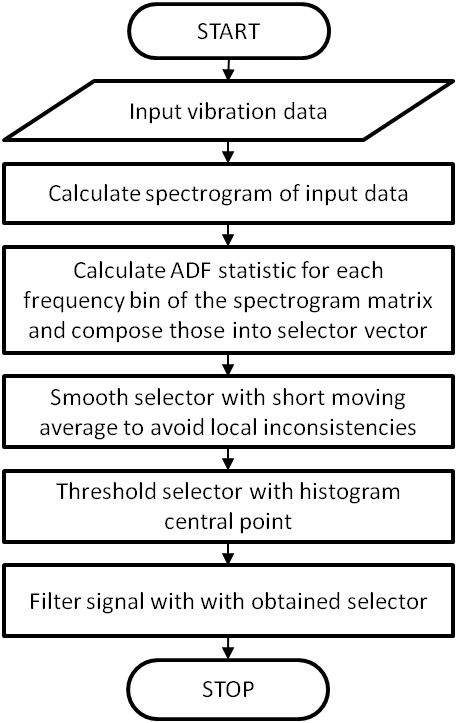
\includegraphics[width=0.48\textwidth]{block}
\caption{Flowchart of the proposed procedure. \label{f:block}}
\end{center}
\end{figure}

First, the spectrogram of the input data is calculated as a time-frequency representation allowing to access narrow frequency bands. Next, for each subsignal of the time-frequency representation the ADF statistic  (see Equation (\ref{eq:spec})) is estimated. It should be mentioned that the ADF test, based on the ADF statistic,  is a classical test often used to test the nonstationarity of real data. Finally the selector is smoothed and thresholded.  In the following subsections the proposed procedure is described in more details.

\subsection{Time-frequency representation}
The procedure begins with the calculation of a spectrogram (see Equations (\ref{eq:spectrogram}) and (\ref{eq:spec})). The spectrogram parameters are selected based on empirical testing taking into account the length of the signal time series. For the specific analyzed real signal (see section 3) the parameters are presented in Table \ref{tab:tab}.

The Short-Time Fourier Transform (STFT) for the discrete signal $y_0, y_1, \dots , y_{N-1}$ is defined as follows \cite{oppenheim1999discrete}:
\begin{equation}
\label{eq:spectrogram}
\textrm{STFT}(t,f)=\sum_{m=0}^{L-1} y_{t+m}\omega_{m}e^{-j2\pi fm/N}
\end{equation}
for $0\leq f\leq f_{max}$ and $0\leq t\leq t_{max}$. In the above equation $\omega$ is a shifted window of length $L$. Furthermore, the spectrogram is estimated as the squared absolute value of the STFT:

\begin{equation}
\label{eq:spec}
\textrm{Spec}(t,f)=|\textrm{STFT}(t,f)|^2.
\end{equation}

\subsection{Augmented Dickey-Fuller (ADF) selector}
The problem of testing stationarity of real data has been widely discussed in the literature. Different approaches applied in this issue can be found. Classical tests are for instance the Dikey-Fuller (DF), the Kwiatkowski-Phillips-Schmidt-Shin (KPSS) and the Durbin-Watson 
\cite{dickey1979distribution,kwiatkowski1992testing,durbin1951testing}. However one of the most popular tests for stationarity is the augmented Dickey–Fuller test (ADF). The null hypothesis of the ADF test is that the unit root is present in the analyzed data, i.e. the data follow the model:
\begin{equation}
    \label{ADF_model}
    y_t=c+\delta t + \phi y_{t-1} + \beta _1 \Delta y_{t-1} + \dots +  \beta _p \Delta y_{t-p} + \epsilon _t,
\end{equation}
where $\Delta$ is the differencing operator, $p$ is the number of lagged difference terms and $
\{\epsilon _t\}$ constitutes a sample of independent identically Gaussian distributed random variables with mean zero and variance $\sigma^2$ $ \left( N(0,\sigma^2) \right) $. The unit root is found when $\phi=1$, i.e. after differentiation, the signal corresponds to an autoregressive process of order $p$ (AR(p)).
In this paper, the authors take under consideration the simpler version with no drift ($c=0$), no trend ($\delta=0$) and (p=0). In this case the model (\ref{ADF_model}) takes the form:
\begin{equation}
    \label{ADF_model_1}
    y_t=\phi y_{t-1} + \epsilon _t,
\end{equation}
which is  an autoregressive model of order 1 (AR(1)) in case $\phi \neq 1$.  In the considered case, the ADF statistic used in ADF test with null hypothesis, defined as in (\ref{ADF_model_1}), is given by:
\begin{equation}
    \label{ADF_stats}
  ADF_{stats}= \frac{ \hat{\phi} }{ se(\hat{\phi}) },
\end{equation}
where $\hat{\phi}$ is the AR(1) coefficient computed by using the Ordinary Least Squares method and $se$ is the standard error of the estimated value. According to the scheme of this procedure, presented in Figure \ref{f:block}, ADF statistics are calculated for each frequency bin from the spectrogram. The ADF selector is set equal to the absolute value of the ADF statistic. 

\subsection{Spectral Kurtosis}

The Spectral Kurtosis has been introduced by Antoni and Randall \cite{ANTONI2006308,ANTONI2006282} and it is considered as one of the most powerful  and popular approaches to localize an Informative Frequency Band (IFB), especially for  vibration signal analysis. The general principle of operation is to calculate the kurtosis value (see Equation (\ref{eq:kurtosis})) for  each  frequency  bin  of  the spectrogram: 

\begin{equation}
\label{eq:kurtosis}
\textrm{Kurt}[Spec(t,f)]=\frac{m_4}{{m_2}^2}=\frac{\frac{1}{n} \sum_{i=1}^{n} \left(y_i - \overline{y} \right)^4}{\left({\frac{1}{n} \sum_{i=1}^{n} \left(y_i - \overline{y} \right)^2}\right)^2},
\end{equation}
where $m_4$ is the fourth central moment, $m_2$ is the second sample moment (sample variance), $y$ is a single time-domain vector corresponding to the given frequency bin $f$ and $0\leq f\leq f_{max}$.

As a result, an indicator of impulsiveness across the signal spectrum can be obtained, allowing to determine which frequency bands carry the most visible information about the damage-related impulsive behavior.  The indicator is named Spectral Kurtosis (SK) and a Vector of SK can be then used as a filter to extract the impulsive components from the signal.

\subsection{Post-processing of ADF selector}
% Smooth and threshold
After obtaining an ADF selector (as well as the SK selector),  it is proposed to post-process it for further enhancement. First, it is smoothed using the moving average with a relatively small window (10 samples in this case) just to eliminate the local variance between the adjacent frequency bands. Afterwards a noise gate is applied by thresholding the smoothed selector with the central point of its histogram. The details of this procedure can be found in \cite{daponte2003ieee}.

As a final step, after the calculation of the proposed ADF selector in function of $f$, which is just an absolute value of the ADF statistic obtained for each subsignal from the spectrogram, the signal can be further filtered.  It is expected that the filtered signal in time domain is more impulsive than the original one. This is related to the fact that the  filter characteristic emphasizes the frequency bands which contain the impulses related to the damage. One of the classical measure of impulsiveness is the kurtosis, therefore this statistic is finally calculated for the envelope of the filtered signal in order to prove the effectiveness of the proposed procedure. As a comparison, the SK selector is calculated also for the original signal and is considered as the filter characteristic. Finally, the kurtosis of the envelope of the SK filtered signal is calculated and is compared to the kurtosis of the envelope of the signal filtered by the ADF filter characteristic. 

\section{Real-life data analysis}

Vibration data have been captured by a commercial measurement system on the rolling ball bearing of the drive pulley operating in a belt conveyor driving station, presented in Figure~\ref{f:rl}. The sensor for measuring the vibration signal was located in the horizontal direction. The sampling frequency is equal to 19 200~Hz. In Figure~\ref{f:raw} are presented 2.5 seconds of raw vibration signals captured over a healthy bearing (top panel) and a faulty bearing (bottom panel).  

\begin{figure}[!ht]
\begin{center}
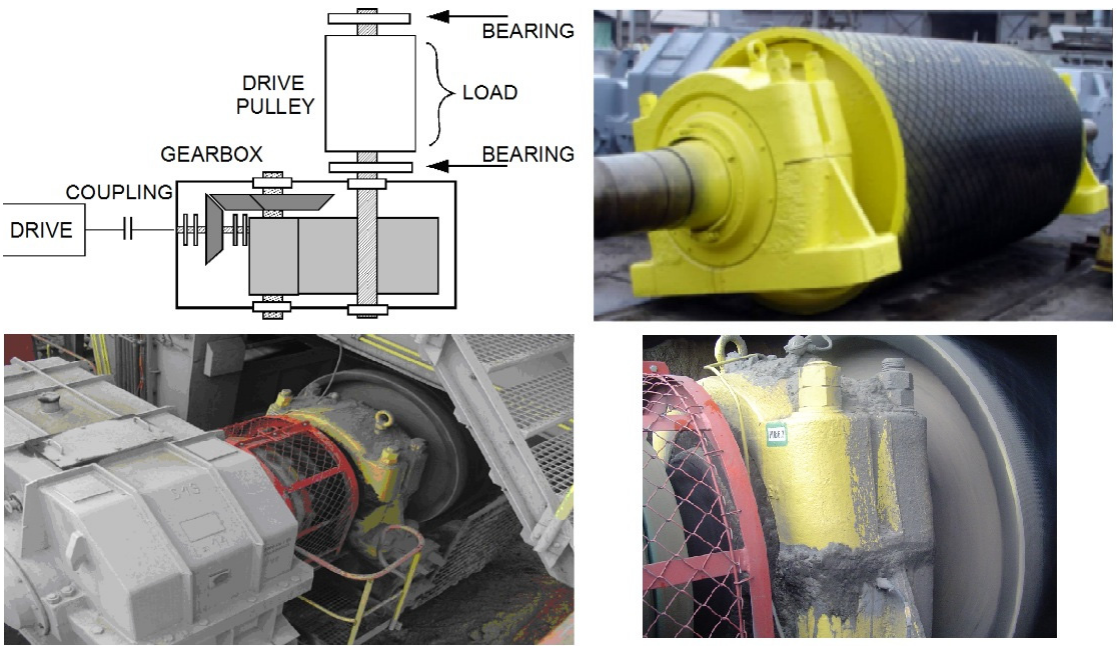
\includegraphics[width=0.9\textwidth]{gb.PNG}
\caption{A drive pulley operating in a belt conveyor driving station \label{f:rl}}
\end{center}
\end{figure}

\begin{figure}[!ht]
\begin{center}
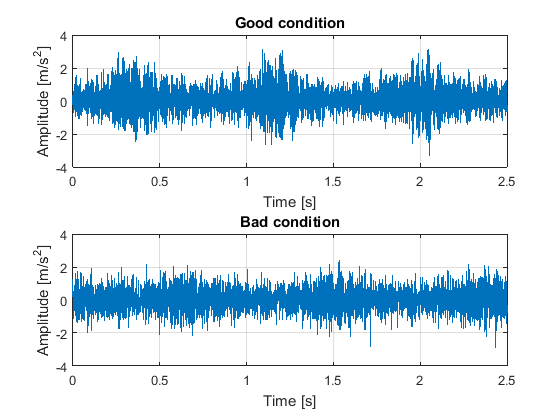
\includegraphics[width=0.85\textwidth]{fig2.png}
\caption{Raw vibration data \label{f:raw}}
\end{center}
\end{figure}

\begin{figure}[!ht]
\begin{center}
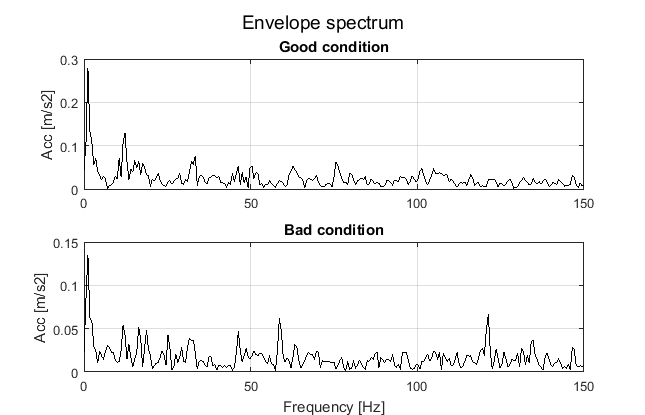
\includegraphics[width=0.8\textwidth]{envelope_raw.png}
\caption{Envelope spectrum of raw vibration data. \label{f:envelope_raw}}
\end{center}
\end{figure}

% \begin{figure}[!ht]
%   \centering
%   \begin{subfigure}[b]{0.48\textwidth}
%       \centering
% %  ?     \captionsetup{skip=0.01pt}
%   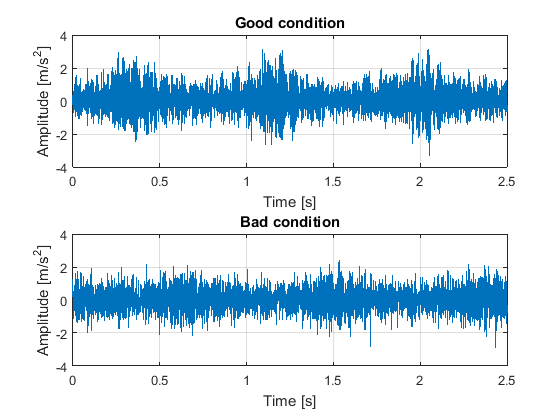
\includegraphics[width=1\textwidth]{fig2.png}
% \caption{Raw vibration data \label{f:raw}}
%   \end{subfigure}
%   %\hfill
%   \begin{subfigure}[b]{0.48\textwidth}
%       \centering
%     %   \captionsetup{skip=0.01pt}
% 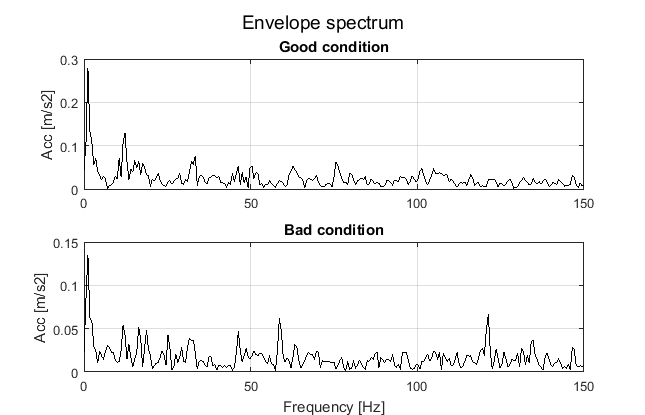
\includegraphics[width=1\textwidth]{envelope_raw.png}
% \caption{Envelope spectrum of raw vibration data. \label{f:envelope_raw}}
%   \end{subfigure}
%   \caption{One-dimensional sample variance of filtered AD map thresholded by local minimum of smoothed histogram of the variance vector}
%   \label{fig:fig_razem}
% \end{figure}

The envelop spectrum of both analysed signals are presented in Figure \ref{f:envelope_raw}. It should be noted, that analysing the raw time signals, it is difficult to observe an impulsive behavior corresponding to the bad (faulty) condition. Moreover the envelope spectrum does not provide clear information about the damage. 

Furthermore, the time-frequency representation (spectrogram) of the signals presented in Figure \ref{f:raw} are shown in Figure \ref{f:spec1}. They have been calculated according to the parameters presented in Table \ref{tab:tab}. 
Some peaks between 1 and 6 kHz are observed at the spectrogram corresponding to the signal from the machine in bad condition. 

\begin{figure}[!ht]
\begin{center}
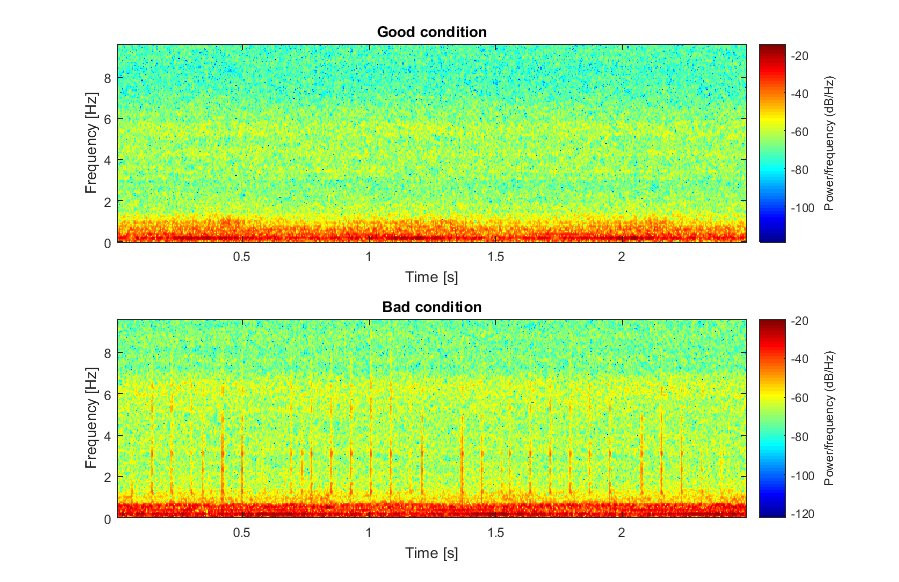
\includegraphics[width=0.8\textwidth]{spec.png}
\caption{Time-frequency representation (spectrogram) of the input data. \label{f:spec1}}
\end{center}
\end{figure}

\begin{table}[ht!]
    \centering
    \caption{Parameters of compared results.}
  \begin{tabular}{|l|l|}
    \hline
    \textbf{Parameter} & \textbf{Value} \\ \hline
         Sampling frequency & 19200 Hz \\ \hline
         Window & Hamming, 256 samples \\ \hline
         Overlap & $60\%$ window \\ \hline
         FFT points & 512 \\
    \hline
    \end{tabular}
    \label{tab:tab}
\end{table}

Next, the ADF statistic for each frequency bin of the spectrogram is calculated. In Figure \ref{f:stats} the values of ADF statistic are presented. 

The values of the statistic are lower for those frequencies for which an impulsive behavior is expected. This indicates that the subsignals corresponding to those frequencies are "more nonstationary" compared to other frequency bands.

\begin{figure}[!ht]
\begin{center}
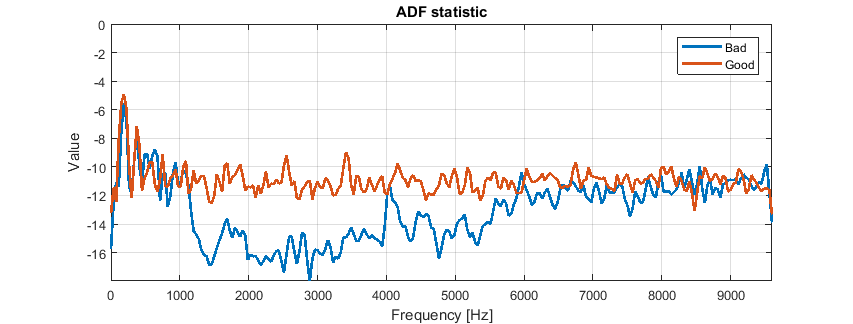
\includegraphics[width=0.8\textwidth]{lozysko_stats1_2.png}
\caption{ADF statistic for signal of the machine in good and bad condition. \label{f:stats}}
\end{center}
\end{figure}

The ADF selector, i.e. the absolute value of the ADF statistic and the corresponding filter characteristic are presented in Figure \ref{f:selector}.

\begin{figure}[!ht]
\begin{center}
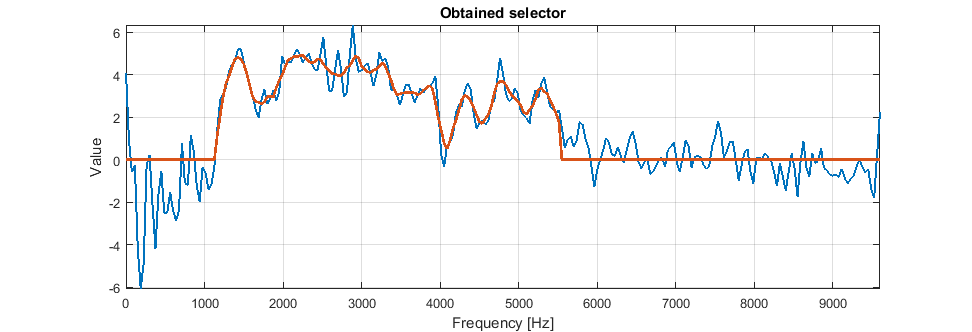
\includegraphics[width=0.8\textwidth]{selector_3.png}
\caption{ADF selector and ADF filter characteristic.\label{f:selector}}
\end{center}
\end{figure}

After its estimation, the filter function is applied over the signals. The filtered signal captured over the machine in a bad condition (using the obtained characteristics) is presented in Figure \ref{f:filtered} while the corresponding spectrogram of the filtered signal is presented in Figure \ref{f:spec_filtered}.

\begin{figure}[!ht]
  \centering
  \begin{subfigure}[b]{0.7\textwidth}
      \centering
%  ?     \captionsetup{skip=0.01pt}
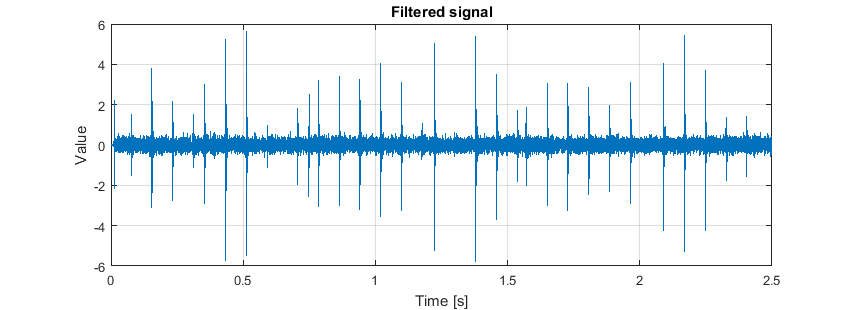
\includegraphics[width=\textwidth]{filtered_signal_2.png}
\caption{Signal after filtration using ADF filter characteristic. \label{f:filtered}}
  \end{subfigure}
  %\hfill
  \begin{subfigure}[b]{0.7\textwidth}
      \centering
    %   \captionsetup{skip=0.01pt}
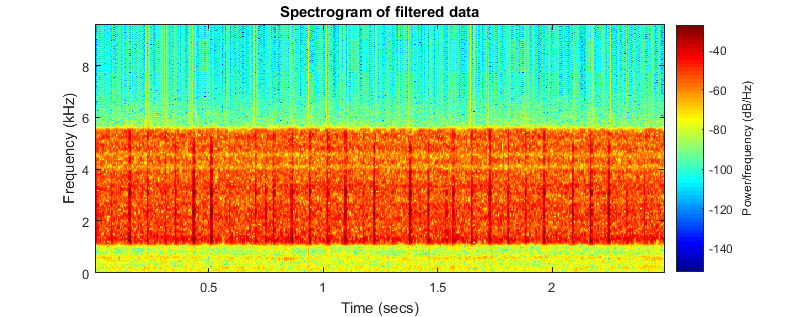
\includegraphics[width=\textwidth]{spec2_1.png}
\caption{Spectrogram of filtered signal. \label{f:spec_filtered}}
  \end{subfigure}
  
    \begin{subfigure}[b]{0.7\textwidth}
      \centering
    %   \captionsetup{skip=0.01pt}
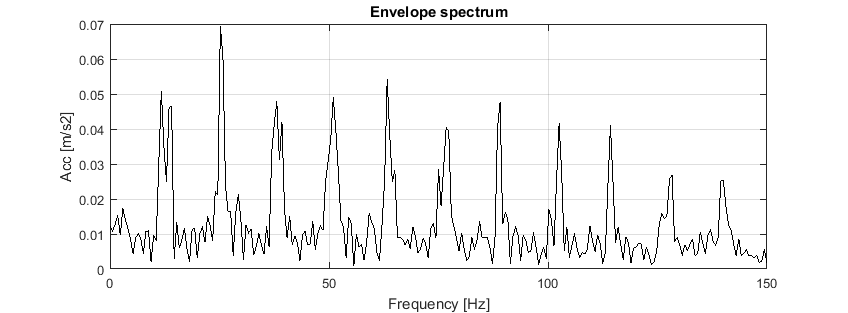
\includegraphics[width=\textwidth]{envelope_2.png}
\caption{Envelope spectrum of filtered signal. \label{f:envelope}}
  \end{subfigure}
  \caption{Presentation of signal in various domains after filtration procedure using obtain selector.}
  \label{fig:fig_razem}
\end{figure}




% \begin{figure}[!ht]
% \begin{center}
% 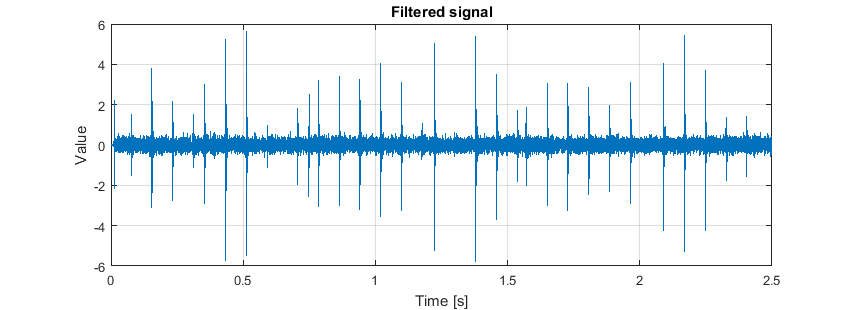
\includegraphics[width=0.8\textwidth]{filtered_signal_2.png}
% \caption{Signal after filtration using ADF filter characteristic. \label{f:filtered}}
% \end{center}
% \end{figure}

% \begin{figure}[!ht]
% \begin{center}
% 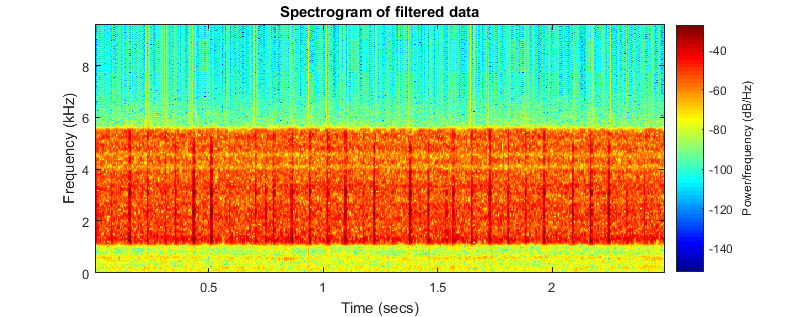
\includegraphics[width=0.8\textwidth]{spec2_1.png}
% \caption{Spectrogram of filtered signal. \label{f:spec_filtered}}
% \end{center}
% \end{figure}

% \begin{figure}[!ht]
% \begin{center}
% 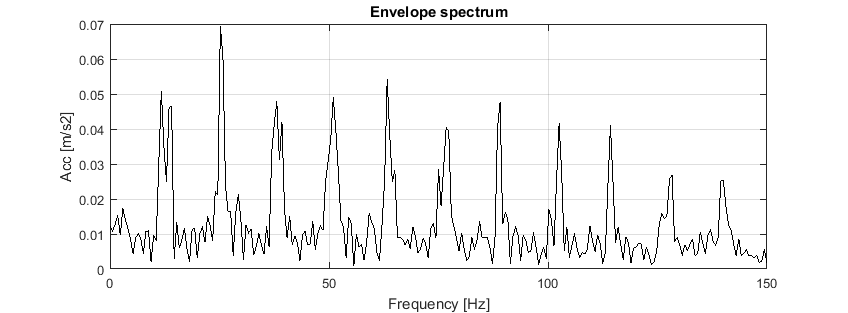
\includegraphics[width=0.8\textwidth]{envelope_2.png}
% \caption{Envelope spectrum of filtered signal. \label{f:envelope}}
% \end{center}
% \end{figure}



Finally the envelope spectrum of the filtered signal is analysed. Comparing Figure \ref{f:envelope_raw} and Figure \ref{f:envelope}, it can be observed that the impulsiveness can be easier detected at the filtered signal compared to the original signal. Moreover, in order to compare the SK- and the ADF- selector results, a similar methodology have been followed for the SK approach. 

More precisely, the SK has been calculated for the raw signal corresponding to the machine in bad condition and the signal is further filtered according to SK characteristic. 

Similar to the ADF statistic, the SK statistic has been also smoothed and thresholded (see the red line in Figure \ref{f:SK}). Finally the kurtosis of the envelope of the filtered signals obtained after using the ADF and the SK approach are compared. The kurtosis of the envelope of the filtered data for the ADF selector has been calculated equal to 88.2290 while for the SK it was calculated equal to 66.7322.

\begin{figure}[!ht]
\begin{center}
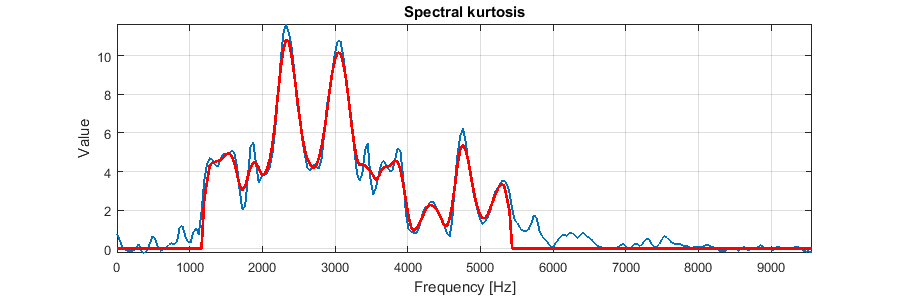
\includegraphics[width=0.8\textwidth]{SK2.png}
\caption{Spectral kurtosis and SK selector. \label{f:SK}}
\end{center}
\end{figure}


\section{Conclusions}
In this paper, a novel method for fault detection in bearings, based on the Augmented Dickey-Fuller (ADF) test has been presented, as an alternative to the classical Spectral Kurtosis approach. The ADF statistic is used as a measure of nonstationarity which results from the impulsive behavior of a signal and further as an Informative Frequency Band selector. The methodology has been applied on a signal captured over a drive pulley operating in a belt conveyor driving station and has been compared to the classical SK approach. Based on this comparison, the new algorithm seems to be more effective compared to the classical SK. 





\section*{Acknowledgments}
The work of R.Zimroz was supported by the statutory grant.
\bibliographystyle{ISMA}
\bibliography{mybibfile}

\end{document}
